%! Author = Dean
%! Date = 12/28/2023

\chapter{Evolucija konvolucijskih neuronskih mreža}\label{ch:evolucija-konvolucijskih-neuronskih-mreza}
Konvolucijske neuronske mreže \emph{KNM} predstavlja ključnu inovaciju u području analize slika i obrade vizualnih podataka.
U posljednjem razdoblju, KNM arhitektura doživjela je značajan tehnološki napredak.
Ovaj napredak omogućio je postizanje rezultata koji su prije bili nezamislivi, često se približavajući ili čak nadmašujući ljudske sposobnosti u određenim zadacima vizualne analize.
Današnje vrijeme karakterizira raznolikost KNM-ova, s različitim arhitekturama koje su prilagođene specifičnim zadatcima.
Svaka arhitektura ima svoje prednosti i mane, a \enquote{Teorem besplatnog ručka} ukazuje na to da nema univerzalno najbolje arhitekture.
Zato ćemo sada malo proći kroz evoluciju konvolucijskih neuronskih mreža od samih početaka pa do danas.

\section{Neocognitron}\label{sec:neocognitron}
Možemo reći da je Neocognitron preteča konvolucijskih neuronskih mreža.
Ova arhitektura je prva uvela pojmove kao što su ekstrakcija značajki (\emph{feature extraction}), konvolucija (\emph{convolution}), i slojevi uzorkovanja (\emph{pooling layers}).
\FloatBarrier
\begin{figure}[h]
    \centering
    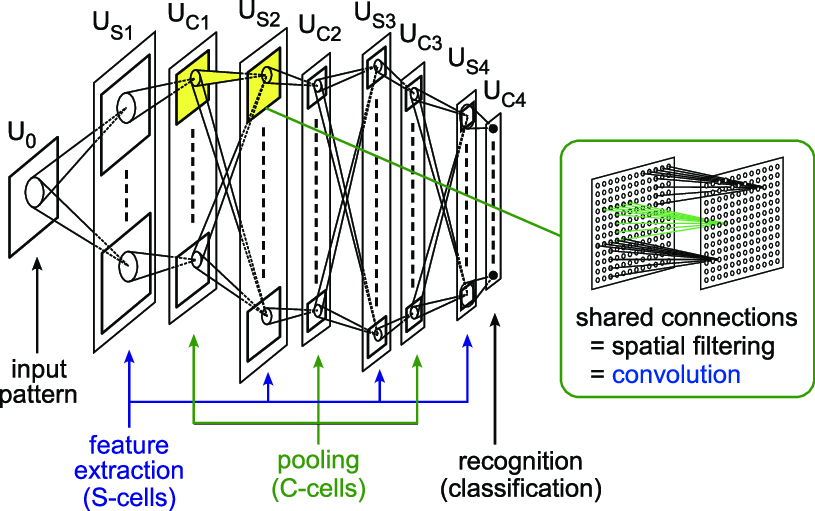
\includegraphics[width=0.6\textwidth]{images/Neocognitron}
    \caption{Arhitektura Neocognitron}
    \label{fig:slika7}
\end{figure}
\FloatBarrier
Arhitektura Neocognitrona sastoji se od alternirajućih S i C slojeva, pri čemu svaki od njih sadrži S i C stanice.
S stanice, ili jednostavne stanice, služe za detekciju lokalnih značajki, dok C stanice, ili kompleksne stanice, služe za dodavanje tolerancije prema samoj poziciji objekta.
Na taj način dobivamo model koji je invarijantan na translacijske promjene, odnosno trebao bi prepoznati oblik bez obzira na to gdje se nalazi na slici.

